%%%%%%%%%%%%%%%%%%%%%%%%%%%%%%%%%%%%%%%%%%%%
\section{AIR4Children}

%%%%%%%%%%%%%%%%%%%%%%%%%%%%%%%%%%%%%%%%%%%%%
\subsection{AIR for Children}

%%%%%%%%%%%%%%%%%%%%%%%%%%%%%%%%%%%%%%%%%%%%%%%%%%%%%%%%
{
\paper{Xochicale M. 2014 \it{Libre Robotics (proposal)} }
\begin{frame}{Prototyping Open Source Robots}
      \begin{figure}
        \centering
        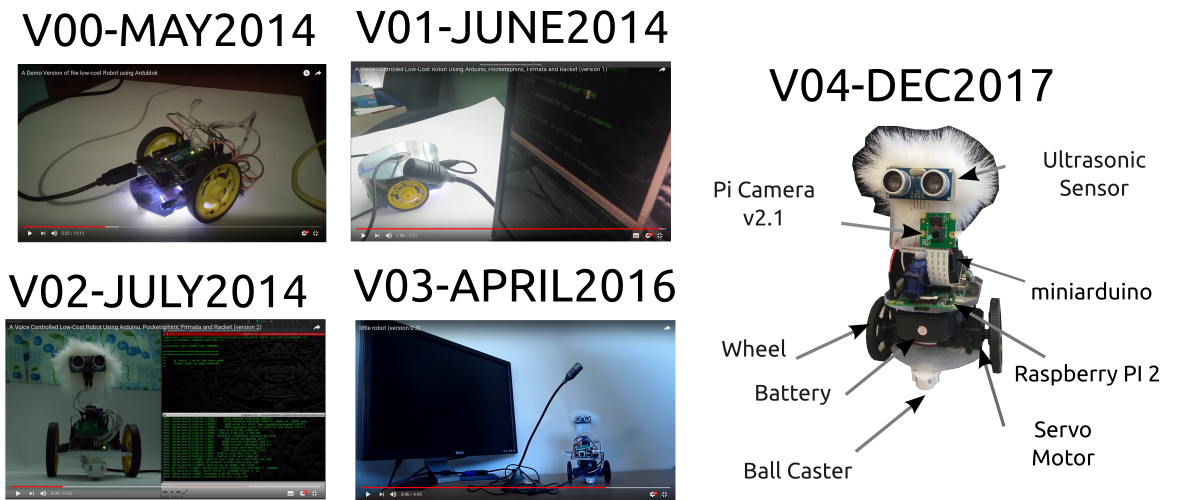
\includegraphics[width=1.0\textwidth]{./figures/air4children/versions/drawing-v00.png}
        %\caption{}
      \end{figure}
\end{frame}
}

%%%%%%%%%%%%%%%%%%%%%%%%%%%%%%%%%%%%%%%%%%%%%%%%%%%%%%%%
{
\paper{Xochicale M. 2015 in Mecate; Parra C. et al. 2016, \it{Otto DIY}}
\begin{frame}{Piloting robot prototypes}
      \begin{figure}
        \centering
        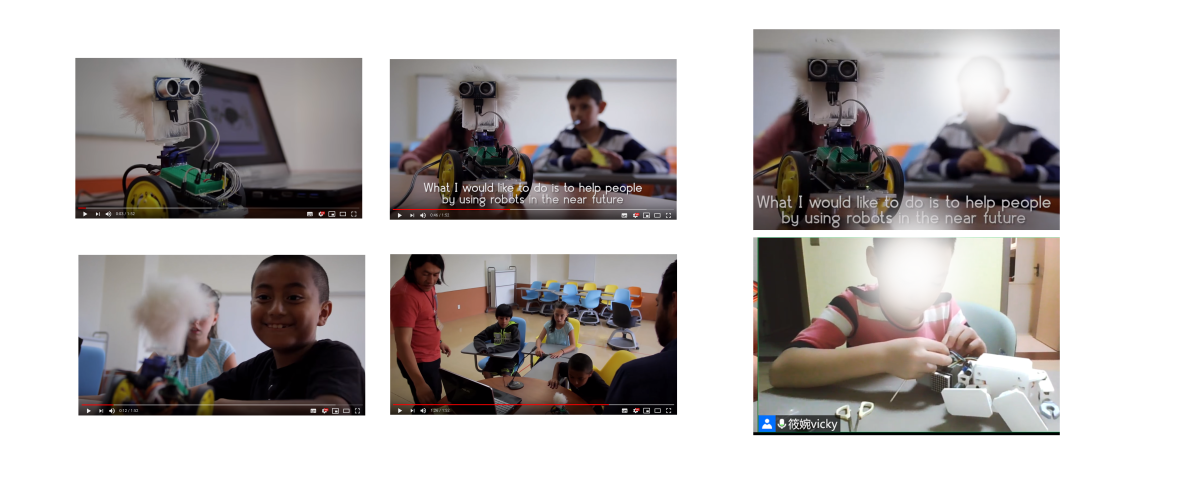
\includegraphics[width=1.0\textwidth]{./figures/air4children/versions/drawing-v01.png}
        %\caption{}
      \end{figure}
\end{frame}
}

%%%%%%%%%%%%%%%%%%%%%%%%%%%%%%%%%%%%%%%%%%%%%
\subsection{Teaching Materials}


%%%%%%%%%%%%%%%%%%%%%%%%%%%%%%%%%%%%%%%%%%%%%%%%%%%%%%%%
{
\paper{Lastname N. YEAR in journal of...}
\begin{frame}{Montessori}

    \begin{figure}
        \centering
        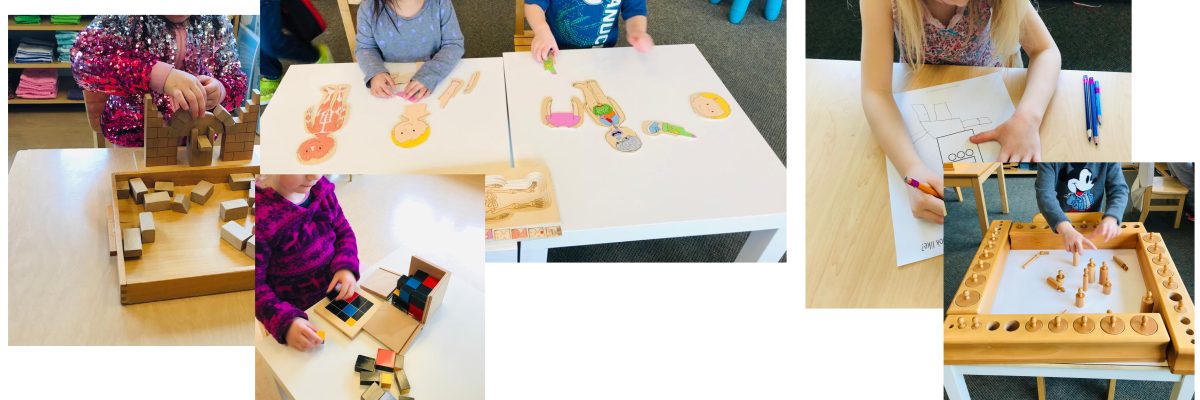
\includegraphics[width=1.0\textwidth]{./figures/montessori/versions/drawing-v00.png}
        %\caption{}
      \end{figure}
\end{frame}
}

%%%%%%%%%%%%%%%%%%%%%%%%%%%%%%%%%%%%%%%%%%%%%%%%%%%%%%%%
{
\paper{Lastname N. YEAR in journal of...}
\begin{frame}{Teaching materials based on Montessori}
* add image that represents montesory skills
      \begin{figure}
        \centering
        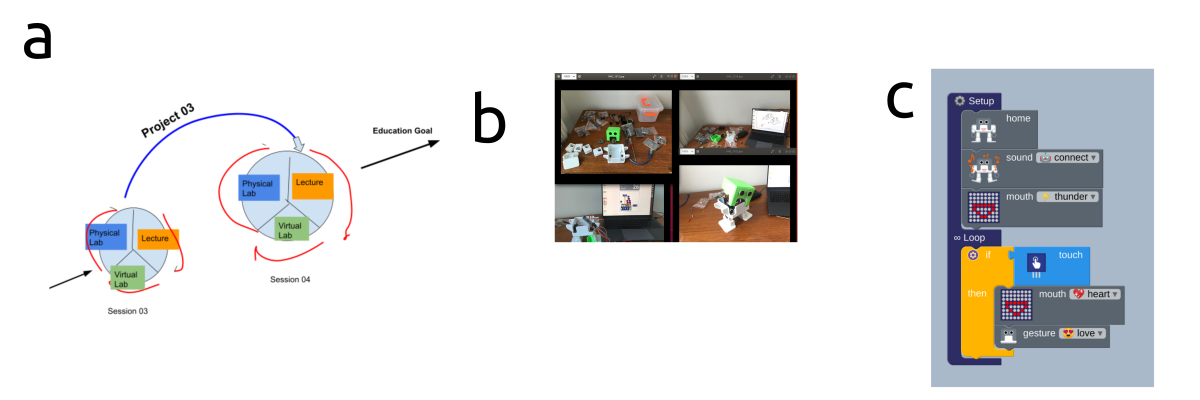
\includegraphics[width=1.0\textwidth]{./figures/teaching-materials/versions/drawing-v01.png}
        %\caption{}
      \end{figure}
\end{frame}
}
